
\section{Geometry Basics}

In this lesson, we will learn how to find the perimeter and area of rectangles, squares and triangles.

\subsection{Rectangle Perimeter}
The perimeter of a rectangle is the total distance around the rectangle's edge. In other words, if you walk along a rectangle's edge once, the distance you will cover is the rectangle's perimeter.

\begin{center}
\begin{tikzpicture}
	\draw (0,0) -- (4,0) -- (4,3) -- (0,3) -- (0,0);
	\draw (0,0.2) -- (0.2,0.2) -- (0.2,0);
	\draw(2,-0.5) node{$4$ inches};
	\draw(-1,1.5) node{$3$ inches};
	\draw(2,3.5) node{$4$ inches};
	\draw(5,1.5) node{$3$ inches};
\end{tikzpicture}
\captionof{figure}{a $4$-inch-by-$3$-inch rectangle}
\label{fig: recPerimeter}
\end{center}

In this figure, we say the \textit{base} of the rectangle is $4$ inches, while the \textit{height} of the rectangle is $3$ inches.

A rectangle's base is also called \textit{length}, and a rectangle's height is also called \textit{width}.

This rectangle's perimeter is:
\[ 4+3+4+3 = 14 \text{ in} \]

In a rectangle, the opposite sides always have the same length. Instead of writing $4+4$, we could write $2\cdot4$; instead of writing $3+3$, we could write $2\cdot3$. So we could calculate a rectangle's perimeter this way:
\[ 2(4+3)=2\cdot7=14 \text{ in} \]

Here is the formula for a rectangle's perimeter:
\[ \text{rectangle perimeter} = 2(\text{base}+\text{height}) \]

\subsection{Square Perimeter}
A square is a special rectangle. A rectangle's opposite sides have the same length, while all four sides of a square have the same length.

\begin{center}
\begin{tikzpicture}
	\draw (0,0) -- (3,0) -- (3,3) -- (0,3) -- (0,0);
	\draw (0,0.2) -- (0.2,0.2) -- (0.2,0);
	\draw(1.5,-0.5) node{$3$ inches};
	\draw(-1,1.5) node{$3$ inches};
	\draw(1.5,3.5) node{$3$ inches};
	\draw(4,1.5) node{$3$ inches};
\end{tikzpicture}
\captionof{figure}{a $3$-inch-by-$3$-inch square}
\label{fig: squPerimeter}
\end{center}

To find the square's perimeter, we simply do:
\[ 
\begin{aligned}[t]
	&\phantom{{}=}\text{square perimeter} \\
	&= 4 \cdot \text{base} \\
	&=4\cdot3 \\
	&=12 \text{ in} 
\end{aligned}
\]

\subsection{Triangle Perimeter}
There is no formula to find a triangle's perimeter---we simply add up the lengths of a triangle's three sides.

\begin{center}
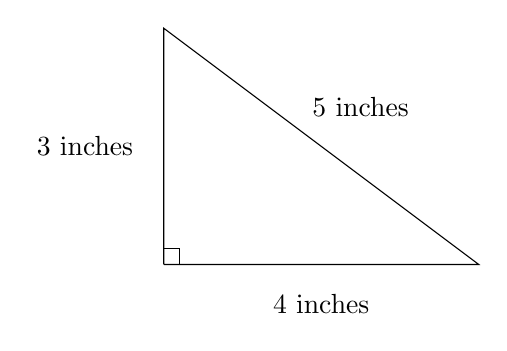
\begin{tikzpicture}
	\draw (0,0) -- (4,0) -- (0,3) -- (0,0);
	\draw (0,0.2) -- (0.2,0.2) -- (0.2,0);
	\draw(2,-0.5) node{$4$ inches};
	\draw(-1,1.5) node{$3$ inches};
	\draw(2.5,2) node{$5$ inches};
\end{tikzpicture}
\captionof{figure}{a triangle}
\label{fig: triPerimeter}
\end{center}

This triangle's perimeter is:
\[ \text{triangle perimeter} = 3+4+5 = 12 \text{ in} \]

\subsection{Rectangle Area}
Earlier, we learned how to find a figure's perimeter---it's the distance around the edge of the figure. Area is a different concept. Let's look at a rectangle cut into small "unit squares." Each unit square's base is $1$ unit in length.

\begin{tightcenter}
   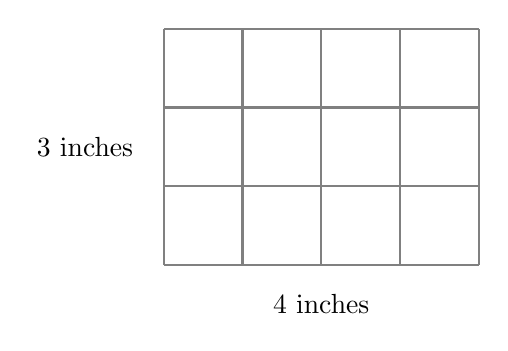
\begin{tikzpicture}
      \draw[step=1.0cm,gray,thick]
      (0,0) grid (4,3);
	\draw(2,-0.5) node{$4$ inches};
	\draw(-1,1.5) node{$3$ inches};
   \end{tikzpicture}
   \captionof{figure}{a $4$-inch-by-$3$-inch rectangle}
   \label{fig: recSquare}
\end{tightcenter}

Each $1$-inch-by-$1$-inch unit square has an area of $1$ square inch. This rectangle has a total of $4 \cdot 3 = 12$ such unit squares, so the rectangle's area is $12$ square inches.

The formula of a rectangle's area is:
\[ \text{rectangle area}=\text{base} \cdot \text{height} \]
or
\[ \text{rectangle area}=\text{length} \cdot \text{width} \]

Note that the unit of this rectangle is "square inch". This is different from the unit of a rectangle's perimeter---inch. The word "square" implies we are dealing with area, not length.

Instead of writing the words "square inches", we could also write $\text{in}^{2}$. Don't confuse this with "square of a number". Let's make a comparison:
\begin{itemize}
\item "$3^{2}$" means "three squared", or $3\cdot3=9$.
\item "$3 \text{ in}^{2}$" means "three square inches", the size of three $1$-inch-by-$1$-inch unit squares.
\end{itemize}

\subsection{Square Area}
A square is a special rectangle, so it's area formula is the same as a rectangle's area formula, except a square's base and height always have the same length. Because of this, instead of writing a square's area formula as $\text{base} \cdot \text{base}$, we can write a square's area formula as

\[ \text{square area} = \text{base}^{2} \]

\begin{myexample}
Find the area of the following square.

\begin{center}
\begin{tikzpicture}
	\draw (0,0) -- (3,0) -- (3,3) -- (0,3) -- (0,0);
	\draw (0,0.2) -- (0.2,0.2) -- (0.2,0);
	\draw(1.5,-0.5) node{$3$ inches};
	\draw(-1,1.5) node{$3$ inches};
	\draw(1.5,3.5) node{$3$ inches};
	\draw(4,1.5) node{$3$ inches};
\end{tikzpicture}
\captionof{figure}{a $3$-inch-by-$3$-inch square}
\label{fig: squArea}
\end{center}
\end{myexample}

\begin{solution}
To find the square's area, we simply do:
\[ \text{square area}=\text{base}^{2}=3^{2}=9 \text{ in}^{2} \]
\end{solution}

\subsection{Triangle Area}
In the following figure, we can clearly see a triangle is half as big as a rectangle with the same base and height.

\pagebreak
\begin{center}
\begin{tikzpicture}
	\draw (0,0) -- (4,0) -- (0,3) -- (0,0);
	\draw (0,0.2) -- (0.2,0.2) -- (0.2,0);
	\draw[dotted] (0,3) -- (4,3) -- (4,0);
	\draw(2,-0.5) node{$4$ in};
	\draw(-0.5,1.5) node{$3$ in};
\end{tikzpicture}
\captionof{figure}{A triangle is half as big as a rectangle.}
\label{fig: triArea1}
\end{center}

To find the area of a triangle, we first find the rectangle's area by $(\text{base})\cdot(\text{height})$, and then divide the rectangle's area by $2$:
\[ \text{triangle area}=\text{base} \cdot \text{height} \div2 \]

The triangle's area in \cref{fig: triArea1} is:
\[ \text{triangle area}=4\cdot3\div2 = 6 \text{ in}^{2} \]

In \cref{fig: triArea1}, the triangle has a right angle ($90$ degrees). It is called a \textit{right triangle}. The same area formula works for non-right triangles.

\begin{center}
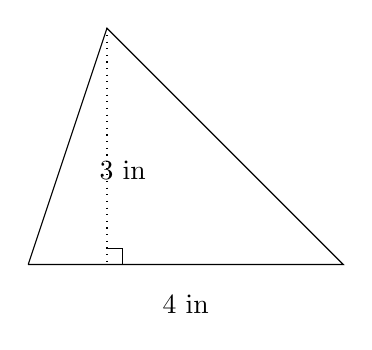
\begin{tikzpicture}
	\draw (0,0) -- (4,0) -- (1,3) -- (0,0);
	\draw[dotted] (1,3) -- (1,0);
	\draw (1.2,0) -- (1.2,0.2) -- (1,0.2);
	\draw(2,-0.5) node{$4$ in};
	\draw(1.2,1.2) node{$3$ in};
\end{tikzpicture}
\captionof{figure}{a non-right triangle}
\label{fig: triArea2}
\end{center}

The triangle's area in \cref{fig: triArea2} is still:
\[ 
\begin{aligned}[t]
	&\phantom{{}=}\text{triangle area} \\
	&= \text{base} \cdot \text{height} \div2 \\
	&=4\cdot3\div2 \\
	&=12\div2 \\
	&=6 \text{ in}^{2} 
\end{aligned}
\]

In \cref{fig: triArea2}, the dotted line is the triangle's \textit{height}. The small square at the bottom of the height implies $90$ degrees. A triangle's height must form a $90$-degree angle with the base.

\subsection{Summary}
Let's review important formulas we learned in this lesson:

\begin{itemize}
\item $\text{rectangle perimeter} = 2(\text{base}+\text{height})$
\item $\text{square perimeter} = 4 \cdot \text{base}$
\item $\text{rectangle area}=\text{base} \cdot \text{height}$
\item $\text{square area}=\text{base}^{2} $
\item $\text{triangle area}=\text{base} \cdot \text{height} \div2$
\end{itemize}

